\section{Theory}
%\begin{figure*}
   % \centering
    %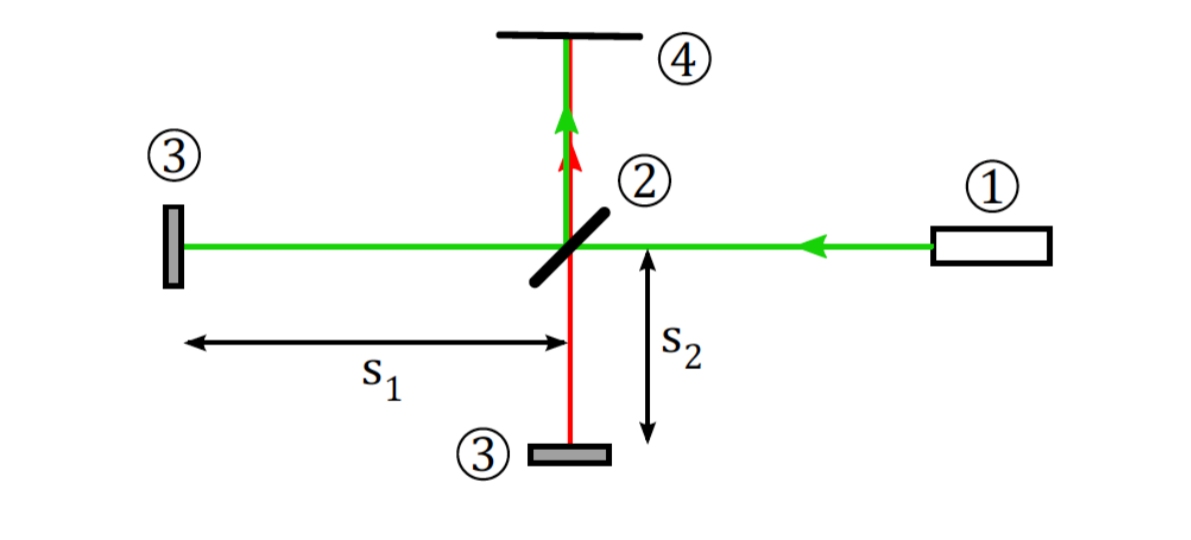
\includegraphics[width=\textwidth]{michelsonsetup}
    %\caption{The simplest setup of a Michelson interferometer.}
   % \label{fig:configuration}
%\end{figure*}
\subsection{Michelson Interferometer}
A Michelson interferometer consist of atleast two mirrors, $m1$ and $m2$, and a beam splitter $m$. A light source $S$ emits light, which is split at the surface of $m$. As $m$ is partially reflective (in our experiment it is assumed to be $50/50$) This ensures that the light is transmitted and reflected equally at the surface of the beamsplitter.

A Michelson interferometer provies a powerful method of measuring the optical properties of a medium. By examining the fringes at the output of a Michelson interferometer one can yield the amplitudes and relative phases of the two beams traversing through reference arm and sample respectively. This holds the information of the optical properties of the medium placed in the sample. The fringes are generated by periodically varying the path length difference between the two arms. This can be done by using a piezo element to oscillate the position of the reference mirror. The mirror oscilattion varies the phase difference between the two beams, often refered to as phase modulation of the instrument.

\subsection{Mach-Zender interferometer}

The Mach-Zender interferometer consist of at least 2 mirrors $m1$ and $m2$ and 2 beamsplitters $b1$ and $b2$. The light from a single source is first split $50/50$ in $b1$, creating a reflected and refracted beam which is lead into $b2$ by mirror $m1$ and $m2$ respectivly. The light reflected and refracted from $b2$ is now a superposition of the light from each arm, thus we will be able to detect an interference pattern, that will depend on the optical path length difference of the arms $\Delta s$. The Mach-Zender interferometer differs from the Michelson Interferometer as the light only transverse each arm once, it does not go forth and back in one arm. 

\subsection{Interference}
%This is probably not arbitrary
Looking at an arbitrary two-arm Interferometer with arms $S_1$ and $S_2$, we will try to describe the intensity $I$ as a function of the path length difference $\Delta s$. Assuming that the light from our laser can be described as a plane wave with an  $\textbf{E}$-field described by:

\begin{align}
\mathbf{E}=\mathbf{E}_0\cos(\omega t-kx)
\label{efelt}
\end{align}

%Where $\mathbf{E_0}$ is a vector which magnitude is the amplitude of our plane wave and with direction of the lights proporgation. $\omega$ is the angular frequency, $t$ is the time, $k=\frac{2\pi}{\lambda}$ is the wavenumber ($\lamba$ is the wavelength of the laser light) and $x$ is the spatial variable. Letting $R$ and $T$ denote the reflection- and transmissioncoefficients for the involved crystals, the beam from our source will first be either reflected or transmitted through it's first interaction, and will then again be either transmitted or reflected after interaction with the second beamsplitter (or second interaction with same beamsplitter). The reflected beam will be transmitted and the transmitted beam will be reflected, which means that we can write the magnitude of our plane wave transversing $S_1$:

\begin{align}
	\mathbf{E_1}=\sqrt{RT}E_0\cos(\omega t+\phi_1)
	\label{Earm}
\end{align}

Where $\phi_1$ is the fase of $S_1$. The expression for the second arm is identical, it only differs with it's own phase $\phi_2$. The intensity of an EM-wave is given by $I=c\varepsilon_0 E^2$. Since the wave in each arm is a superposition of the wave from $S_1$ and $S_2$ the intensity of the interferometer output will be:

\begin{align}
I = c\varepsilon_0 |\mathbf{E_1}+\mathbf{E_2}|^2=c\varepsilon_0 RTE_{0}^2 (\cos(\omega t +\phi_1)+\cos(\omega t+\phi_2))^2
\label{intensity1}
\end{align}

Since the light oscillates relatively rapidly, we only observe the time averaged intensity in our detector. Taking the time average of the intensity we get:

\begin{align}
\bar{I}=c\varepsilon_0 RTE_{0}^2(1+\cos(\phi_1-\phi_2))
\label{intensityav1}
\end{align}

Assuming that $R=T=\frac{1}{2}$ and renaming the phase difference $\Delta \phi=\phi_1-\phi_2$, we can write the average intensity:

\begin{align}
\bar{I}=\frac{1}{4}c\varepsilon_0 E_{0}^2(1+\cos(\Delta \phi))
\label{intensityav2}
\end{align}

Where the phase differences translates linearly to the path length difference with the wave number as propertionality constant e.g.:

\begin{align}
\Delta \phi = \frac{2\pi}{\lambda}\Delta s
\label{phasetrans}
\end{align}



\subsection{}<++>

\subsection{Piezo Electric Crystal}
%\fxme{Driven frequency, is it a resonance? Maximal displacement?}

A piezo electric material has the property that it contracts or expand when a voltage is applied over the material, and likewise compressing or stressing the material will induce a voltage over the material. The displacement of the piezoelectric component is linearly proportianel to the voltage applied over the material:

\begin{align}
d = c_{piezo}\Delta V
\label{piezodisp}
\end{align}

Where the piezo-electric constant $c_{piezo}$ is a material constant.\\

In relation to our experiment we are going to compare the detected intensity $I$ of our beam with a periodically changing voltage $\Delta V$. Our raw data will be a $(t,I)$-graph and a $(t, \Delta V)$, by plotting the voltage over half a period with the corresponding intensities for the time we get a $(\Delta V,I)$-graph. The effective change in optical path distance, will correspond to two times the magnitude of the displacement of our piezo-electric material, as we are using the Michelson Interferometer to this exercise. This means that $\Delta s = 2 c_{piezo} \Delta V$. Tracking the the "voltage wavelength" between two peaks $\lambda_V$ on the $(\Delta V,I)$-graph then has to be linearly proportional to the wavelength of \ref{intensityav2} which is $\lambda$ we have:

\begin{align}
\frac{\lambda}{2} = c_{piezo}\lambda_V
\label{piezo}
\end{align}
'
From which we can determine the piezo-electric constant. 

\subsection{Change of refractive index in Mach-Zender Interferometer}

In the experiment where we will be using changing the pressure in a glass tube (6cm) to change our path length. The change pressure in the tube $\Delta p$ is linearly proportional to the change in the refractive index of the medium in the tube $\Delta n$ with a proportionality constant $k$:

\begin{align}
\Delta n = k \Delta p
\label{pn}
\end{align}

A change in the refractive index will change the effective optical path distance, because the speed of light in a given medium $v_i$ is given as $v_i=\frac{c}{n_i}$ with vacuum having an refractive index of $n=1$. In a setup were the surroundings have refractive index $n_1$ and there is a tube of length $s_0$ constructed of a material with refractive index $n_2$, the time it would take a laser beam to pass the length of the tube would differ from the time it would take the laser beam in the surrrounding material. Letting $v_2$ be the speed of light in the tube, $v_1$ the speed of light in the surrounding material, $t_1$ the time it takes the light to transverse $s_0$ in medium 2, and $t_2$ the time it takes the light to transverse $s_0$ in medium 2 (the tube), we have:

\begin{align}
s_0=v_1 t_1
\label{1}
\end{align}

\begin{align}
s_0 = v_2 t_2
\label{2}
\end{align}

Equating \ref{1} and \ref{2}:

\begin{align}
v_1 t_1 = v_2 t_2 \Rightarrow t_2 = \frac{v_1}{v_2}t_1
\label{t2}
\end{align}

We can now compute the difference in time it takes the light to transverse $s_0$:

\begin{align}
\Delta t = t_2-t_1 = (\frac{v_1}{v_2}-1)t_1 = (\frac{n_2}{n_1}-1)t_1=\frac{n_2-n_1}{n_1}t_1
\label{deltat}
\end{align}

This difference in time is the same as the light in medium 1 travelling an effective length of $s_eff=s_0+\Delta s$ where $\Delta s = v_1 \Delta t$ thus we get:

\begin{align}
\Delta s = v_1\frac{n_2-n_1}{n_1}t_1=\frac{n_2-n_1}{n_1}s_0 \Rightarrow n_1\Delta s = \Delta n s_0
\label{sn}
\end{align}

The raw data from the experiment will be the interference pattern observed by our detector as we raise and/or lower the pressure with $\Delta p$. The output will be an $(t,I)$-graph where we can count the number of periods the intensity takes during the change in pressure $m$. The intensity must hae the same number of oscillations if we look at is as a function of optical path difference, thus the total optical path difference obtained by changing the pressure to $\Delta p$ is:

\begin{align}
\Delta s = m\lambda
\label{delsmz}
\end{align}

Using \ref{delsmz} and \ref{sn} we obtain an expression for $\Delta n$

\begin{align}
m\lambda n_1 = \Delta n s_0 \Rightarrow \Delta n = \frac{m \lambda n_1}{s_0}
\label{deln}
\end{align}



